\documentclass[10pt]{article}
\usepackage{icmlko}

\icmlmeta{IP 파운데이션 월드모델}{133}{기준선을 바꾸면 부호가 바뀐다}{팝업 표본을 넓히는 것이 이득인지 손해인지 --- 한 시간 안에 두 번 뒤집혔고, 뒤집은 것은 자료가 아니라 무엇과 견줬느냐였다}

\begin{document}

\twocolumn[
\icmlheader

\begin{abstract}
노트 132가 팝업의 병목을 2025년 이전 레코드 16건으로 확정했다. 노트 127에
그 벽을 넘는 측정이 이미 있었다 --- 계수 방법 필터를 풀어 organizer\_claim
까지 넣으면 이전 이력이 16건에서 73건이 되고, 분모를 고정해도 팝업
$\rho$가 $+$0.3688에서 $+$0.4495로 오른다. 채택하지 않고 넘어갔던 것을
이번에 하네스에 정식으로 붙였다. \textbf{그런데 처음 잰 값은 손해였다}
--- 넓힌 판이 $+$0.4995에서 $+$0.4130으로 내렸다. 원인이 셋 있었고 셋 다
내 쪽이었다. ① 넓힌 팝업에 검색·달력 값을 안 붙이고 중립으로 채워서 넓힌
판이 \emph{정보가 더 적었다}. ② 분모를 (라벨, 시간)으로 맞췄는데 두 경로가
시간을 다르게 계산해 0건이 맞았다. ③ 라벨을 float32로 캐스팅하는 경로가
있어 정확 비교가 1건만 맞았다. 셋을 고치고 \textbf{같은 코드 경로}로
견주니 부호가 뒤집혔다 --- 부스팅 $+$0.3690 $\to$ $+$0.4202, 짝 순위
$+$0.3698 $\to$ $+$0.4300, 직접 풀링 $+$0.3698 $\to$ $+$0.4173.
\textbf{확장은 이득이다}($+$0.048$\sim$$+$0.060, 셋 다). \textbf{그런데
이득의 출처를 갈라 보니 채택할 것은 확장이 아니었다} --- 주장 라벨은
$\rho$ 0.02$\sim$0.07로 예측이 안 되고, 짝 순위 우도는 학습 문턱을 40에서
15로 낮춰 \emph{검증된} 16건만 넣어도 같은 $+$0.4300을 얻는다. 그리고 그 길에
뜻밖의 것을 봤다. 노트 124가 ``사람이 안 매긴 것''이라 판정한 팝업 8건의
마스크를 내리면 팝업 $\rho$가 $+$0.4995에서 $+$0.3698로 \emph{내린다}.
값은 어차피 중립이라 바뀌는 것은 관측 표시자뿐인데, \textbf{``모른다''고
표시하는 것이 ``중립이라고 관측했다''고 두는 것보다 나쁘다.}
\end{abstract}
]

\begin{figure*}[t]
\centering
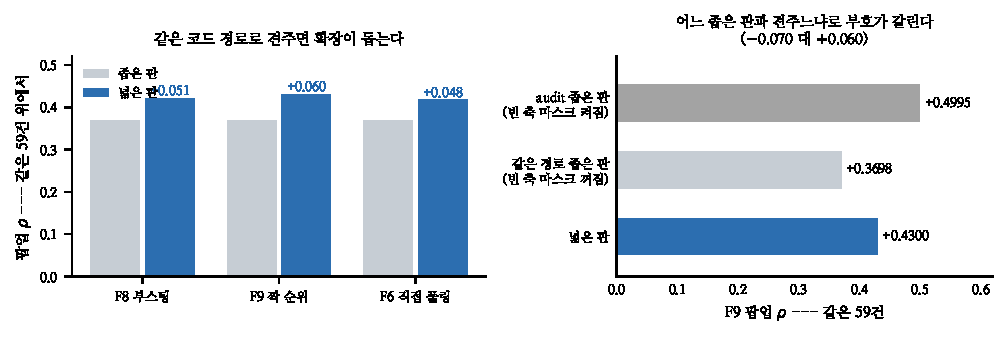
\includegraphics[width=\textwidth]{figs/wide.pdf}
\caption{왼쪽 --- 같은 코드 경로로 견주면 확장이 셋 다 돕는다.
오른쪽 --- 어느 좁은 판과 견주느냐로 같은 확장이 $-$0.070이 되기도
$+$0.060이 되기도 한다.}
\end{figure*}

\section{이미 잰 것을 안 쓰고 있었다}

노트 127이 팝업 표본을 넓히는 세 갈래를 재고 분해까지 해 놓았다.

\begin{table}[t]
\centering\tsize
\caption{노트 127의 분해 --- 분모를 원래 59건에 고정.}
\begin{tabular}{lrl}
\toprule
& $\rho$ & 팝업이 학습에? \\
\midrule
현행 & $+$.3688 & 아니오 \\
현행 · 문턱 15 & $+$.3814 & 예 \\
$+$주장 (이전 73건) & \textbf{$+$.4495} & 예 \\
$+$주장 · 팝업 뺌 & $+$.3244 & 아니오 \\
\bottomrule
\end{tabular}
\end{table}

이득이 ``레코드가 늘어서''가 아니라 ``팝업이 학습 풀에 들어가서''라는 것도
그때 확인했다. 그런데 채택하지 않고 노트 128의 검색 축으로 넘어갔다.
노트 132가 병목을 다시 그 16건으로 짚고 나서야 돌아왔다.

\section{처음 잰 값은 손해였다}

하네스에 자료 갈래로 붙이고(\texttt{--axes wide\_trendcal}) 쟀더니 팝업이
$+$0.4995에서 $+$0.4130으로 내렸다. 노트 127과 정반대다.

원인이 셋이었고 셋 다 내 쪽이었다.

\claimx{\textbf{① 넓힌 판이 정보가 더 적었다.} 부가 축(검색 · 달력)을
좁은 팝업 기준으로 만들어 놓고, 넓힌 팝업 행에는 중립 0.5 · 표시자 0으로
채웠다. 검색 관측률이 0.89에서 \textbf{0.00}이 됐다. 축 생성기가 넓은 id
목록을 쓰도록 고쳤다.}{\texttt{harness.load} 가 행 수가 안 맞는 축을 조용히
중립으로 채우는 설계라 눈에 안 띄었다. 조용히 채우는 대신 경고를 내는 편이
나았을 것이다.}

\claimx{\textbf{② 분모가 0건 맞았다.} 두 경로가 시간을 다르게 계산한다
--- 하나는 연도 정수, 하나는 소수 연도다. (라벨, 시간) 쌍으로 맞추니
59건 중 0건이 맞았다.}{라벨만으로 맞추도록 바꿨다. 같은 라벨이 둘 이상이면
순서대로 소진한다.}

\claimx{\textbf{③ 라벨이 float32와 float64로 갈려 있었다.}
\texttt{load\_popup} 이 \texttt{y.astype(np.float32)} 로 캐스팅한다. 1e-9
허용오차로 맞추니 59건 중 1건만 맞았다. 소수 다섯 자리로 반올림해
해결했다.}{그 전에 ``audit 이 라벨을 변환한다''고 잘못 읽고 변환식을
찾느라 시간을 썼다. 변환이 아니라 정밀도였다.}

\section{고치고 나니 부호가 뒤집혔다}

\begin{table}[t]
\centering\tsize
\caption{같은 코드 경로 · 같은 59건 위에서. 판 $\rho$는 참고.}
\begin{tabular}{lrrr}
\toprule
& 좁은 판 & 넓은 판 & 차 \\
\midrule
F8 부스팅 & $+$.3690 & \textbf{$+$.4202} & $+$.0512 \\
F9 짝 순위 & $+$.3698 & \textbf{$+$.4300} & $+$.0601 \\
F6 직접 풀링 & $+$.3698 & \textbf{$+$.4173} & $+$.0475 \\
\bottomrule
\end{tabular}
\end{table}

\claimx{\textbf{확장은 이득이다.} 정식화 셋 모두 $+$0.048$\sim$$+$0.060.
노트 127이 맞았고, 처음의 ``손해''는 비교가 틀린 것이었다.}{판 $\rho$는
거의 안 움직인다(F8 $+$0.4318 $\to$ $+$0.4217, F9 $+$0.3546 $\to$
$+$0.3527) --- 팝업은 아홉 대상 중 하나이고 넓힌 팝업의 채점 집합
116건 자체가 더 어렵기 때문이다. \textbf{이득은 제품 지표에 있지 판에는
없다.}}

\section{그런데 기준선이 답을 바꾼다}

같은 확장인데 무엇과 견주느냐로 부호가 갈린다.

\begin{table}[t]
\centering\tsize
\caption{F9 팝업 $\rho$, 전부 같은 59건.}
\begin{tabular}{lr}
\toprule
audit 좁은 판 (빈 축 마스크 켜짐) & $+$.4995 \\
같은 경로 좁은 판 (빈 축 마스크 꺼짐) & $+$.3698 \\
넓은 판 & $+$.4300 \\
\bottomrule
\end{tabular}
\end{table}

넓은 판을 첫 줄과 견주면 $-$0.070, 둘째 줄과 견주면 $+$0.060이다.
\textbf{자료도 모형도 그대로인데 결론이 반대가 된다.}

두 좁은 판의 차이는 하나뿐이다. 노트 124가 ``열 축이 전부 상수 2.0이라
사람이 안 매긴 것''이라 판정한 팝업 8건을, 하나는 관측으로 두고 하나는
마스크를 내린다. 축 \emph{값}은 어차피 중립(0.5)이라 같고, 바뀌는 것은
관측 표시자뿐이다.

\claimx{\textbf{``모른다''고 표시하는 것이 ``중립이라고 관측했다''고 두는
것보다 나쁘다.} 마스크를 내리면 팝업 $\rho$가 $+$0.4995에서 $+$0.3698로
0.13 내린다. 표시자를 켜 두면 그 열이 상수라 아무 정보도 안 주는데,
내리면 열이 변하면서 모형이 거기서 무언가를 배우고 그것이 지평 너머에서
해가 된다.}{여덟 건의 사례다. 그리고 노트 124의 판정(``안 매겼다'')이
틀렸다는 뜻은 아니다 --- 그 판정은 맞고, \emph{그 사실을 모형에 알리는
것}이 손해라는 것이다.}

이것이 이번 노트에서 제일 불편한 결과다. 정직하게 결측을 표시하는 쪽이
점수가 낮다. 다만 그 낮음이 ``정직해서 손해''인지 ``여덟 건에서 우연히''
인지는 이 표본으로 안 갈린다.

\section{그리고 가드가 걸렸다 --- 걸린 것은 가드였다}

넓은 판을 정식 라운드에 올리자 \textbf{엿보기 가드가 실패}했다. 대상 라벨을
섞으면 예측이 안 변해야 하는데 최대 1.14 움직였다.

\claimx{\textbf{가드가 틀렸다.} 엿보기는 대상 라벨을 \emph{통째로} 섞었다.
그러면 이력이 충분해서 학습 풀에 정당하게 들어간 도메인은 무조건 실패한다
--- 그 도메인의 $T$ 이전 라벨은 써도 되는 것이다. 팝업 이력을 16건에서
73건으로 넓히자마자 걸렸고, 걸린 쪽이 자료가 아니라 가드였다. $T$ 이후만
섞도록 고치니 넷 다 통과한다.}{이 버그는 팝업이 한 번도 학습 풀에 못
들어갔던 덕에 스물여덟 노트 동안 잠들어 있었다. \textbf{가드는 걸릴 일이
생겨야 검정된다.}}

\section{주장 라벨은 예측이 안 된다}

넓은 판의 후행 116건을 계수 방법으로 갈라 채점했다. 노트 124가 미검정으로
남긴 라벨 품질의 첫 직접 측정이다.

\begin{table}[t]
\centering\tsize
\caption{같은 모형, 같은 예측. 후행 116건을 계수 방법으로 가른 것뿐.}
\begin{tabular}{lrr}
\toprule
& 검증 계수 (59) & 주장 · 추정 (57) \\
\midrule
F8 부스팅 & $+$.4202 & $+$.0715 \\
F9 짝 순위 & $+$.4300 & $+$.0297 \\
F6 직접 풀링 & $+$.4173 & $+$.0199 \\
\bottomrule
\end{tabular}
\end{table}

\claimx{\textbf{organizer\_claim 라벨은 예측이 안 된다} --- $\rho$ 0.02$\sim$0.07
이다. 같은 모형이 검증 계수는 $+$0.42로 맞히는데 주장은 못 맞힌다.}{``라벨이
나쁘다''와 ``그 팝업들이 원래 어렵다''를 이 자료로는 못 가른다. 다만 축과
달력은 두 무리가 같은 방식으로 붙어 있다.}

\section{그러면 확장의 이득은 어디서 왔나}

주장 라벨이 예측 불가라면, 그것으로 학습해서 검증 계수가 좋아질 이유가
없다. 그래서 이득의 출처를 갈랐다 --- 학습 문턱을 40에서 15로 낮추면
주장 레코드 없이도 팝업의 \emph{검증된} 16건이 학습 풀에 들어간다.

\begin{table}[t]
\centering\tsize
\caption{전부 같은 59건 위에서.}
\begin{tabular}{lrr}
\toprule
& F8 부스팅 & F9 짝 순위 \\
\midrule
좁은 · 문턱 40 (팝업 학습 밖) & $+$.3690 & $+$.3698 \\
좁은 · 문턱 15 (검증 16건만) & $+$.3307 & \textbf{$+$.4300} \\
넓은 · 문턱 40 (주장까지 73건) & \textbf{$+$.4202} & $+$.4300 \\
\bottomrule
\end{tabular}
\end{table}

\claimx{\textbf{짝 순위 우도는 검증된 16건만으로 이득 전부를 얻는다.}
$+$0.4300으로 넓은 판과 \emph{똑같다}. 주장 레코드 114건이 더하는 것이
없다.}{부스팅은 다르다 --- 문턱만 낮추면 오히려 $+$0.3307로 내리고 넓은
판에서만 $+$0.4202가 된다. 트리는 16행으로 못 배운다.}

\section{채택}

\claimx{\textbf{학습 문턱을 40에서 15로 낮춘다.} 한 줄이고, 잡음 라벨을
하나도 안 들이고, 짝 순위 우도가 이득 전부를 얻는다. 넓은 판은 트리 계열을
위한 갈래로 남긴다.}{첫 양수를 보고 바로 채택했다면 주장 레코드 114건을
들이는 쪽을 골랐을 것이다. \emph{어디서 왔는지}를 갈라 보니 그럴 필요가
없었다.}

넓은 판을 기본으로 삼지 않는 이유가 하나 더 있다. 그 판의 채점 집합 116건
중 57건이 $\rho$ 0.03으로 예측 불가라, 판 위의 팝업 수치가 $+$0.24로
떨어진다. \textbf{못 맞히는 것을 분모에 넣으면 지표가 무엇을 말하는지
흐려진다.}

\begin{table}[t]
\centering\tsize
\caption{남은 것.}
\begin{tabular}{ll}
\toprule
문턱 15 & 다른 도메인에도 영향 --- 전 판으로 다시 재기 \\
주장 라벨 & 실측 대조가 있어야 ``나쁘다''를 확정한다 \\
마스크 & 여덟 건 사례 --- 표본이 늘면 다시 \\
\bottomrule
\end{tabular}
\end{table}

문턱을 낮추면 팝업만 들어오는 것이 아니다. 아이돌(2025년 이전 54건)은
이미 들어와 있지만 다른 도메인의 경계도 움직일 수 있다. \textbf{채택은
전 판을 다시 재고 확정한다.}

\end{document}
